\documentclass[9pt,a4paper]{article}
\usepackage[utf8]{inputenc}
\usepackage{amsmath,amssymb}
\usepackage[catalan]{babel}
\usepackage{geometry}
\usepackage{hyperref}
 \geometry{
 a4paper,
 total={170mm,257mm},
 left=15mm,
 top=15mm,
 }
\usepackage{graphicx}
\usepackage{authblk}
\usepackage{wrapfig}


\setlength{\parindent}{0pt}


\begin{document}


\title{Creació d'un servidor a Github i control de versions amb RStudio}
\author[]{Aida Fernández Olivares}
\date{}

\maketitle

\section{Que és GitHub?}
Github és una plataforma per a l'allotjament de codis, per al control de versions i la col·laboració. De manera que permet que diversos individus treballin junts en projectes cadascú des del seu dispositiu.

\noindent\rule{\textwidth}{0.5pt}

\section{Descarregar Git}
Git és un sistema de control de versions. Un sistema de control de versions ens va a servir per treballar en equip d'una manera molt més simple i òptima quan estem desenvolupant programari. Quan vam acabar de desenvolupar el nostre codi, fem servir Git per barrejar els canvis amb els altres companys.\\

El primer que haurem de fer és descarregar $git$ per al nostre sistema operatiu:\\
\url{https://git-scm.com/download}\\

Un cop descarregat executarem el fitxer $.exe$ i farem la instalació de manera predeterminada.

\noindent\rule{\textwidth}{0.5pt}

\section{Creació del servidor a Github}
Primer de tot haurem de crear un compte \url{https://github.com/}.\\

Un cop creat, entrarem al nostre compte \url{https://github.com/login}\\

\begin{wrapfigure}{l}{0.65\textwidth}
	\centering
	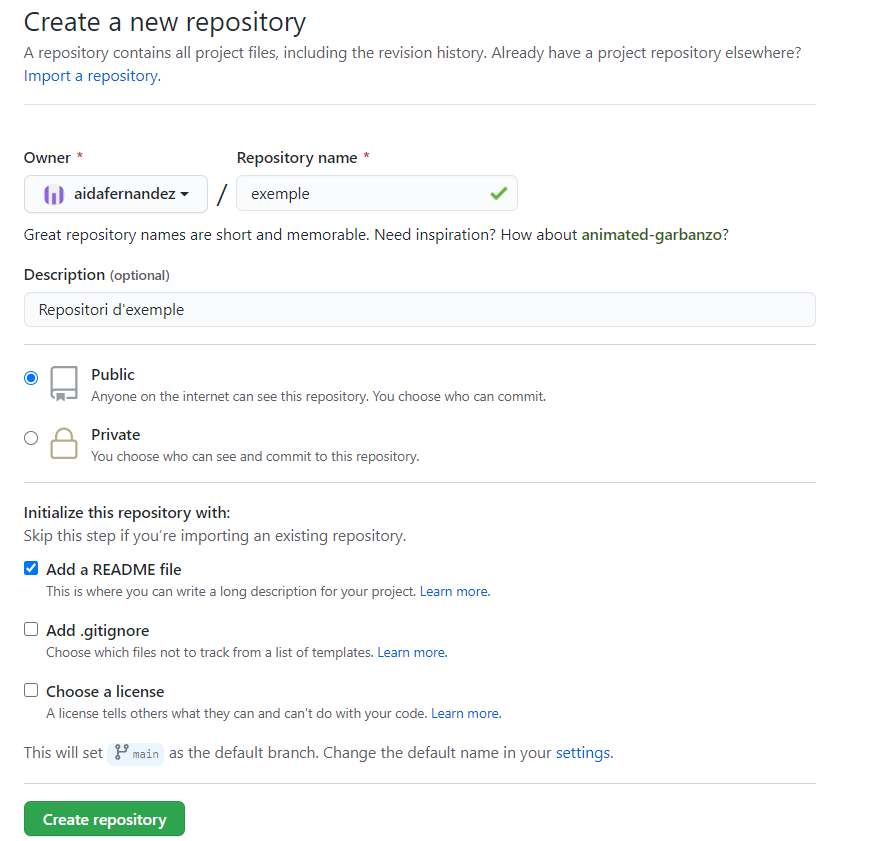
\includegraphics[width=11cm]{create}
\end{wrapfigure}

Ara el que farem serà crear un nou repositori a \url{https://github.com/new}.
Haurem d'elegir un nom (sense espais) i si volem podem afegir una descripció.\\
També haurem d'elegir si volem que sigui un repositori públic (qualsevol persona pot veure el repositori però nosaltres elegim qui pot contribuir-hi) o privat (elegim qui pot veure i contribuir al repositori). \\
Finalment afegirem un fitxer README, és útil a l'hora d'afegir descripcions més extenses del repositori i a més, així el nostre repositori no estarà buit de primeres.\\

Observem el següent exemple:

\clearpage

\section{Pujada d'arxius al repositori}
Un cop creat el repositori s'ens obrirà al github. \\\\
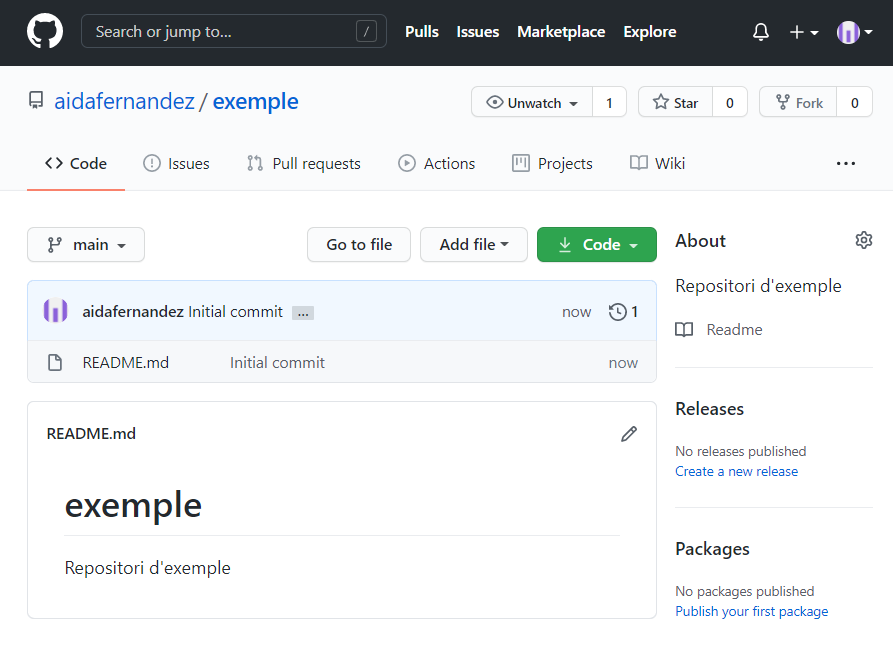
\includegraphics[width=12cm]{repo}\\
Observem que de moment només hi ha el fitxer README.md que s'ha creat automàticament.\\

La manera més sencilla d'afegir arxius és a \url{https://github.com/aidafernandez/exemple/upload/main}.
Simplement haurem d'arrosegar els arxius que volguem afegir al repositori i afegir una breu descripció.


\clearpage
%%%%%%%%%%%%%%%
%%%
%%% References
%%%
%%%%%%%%%%%%%%%
\begin{thebibliography}{x}
\bibitem{}
\url{https://guides.github.com/activities/hello-world/}

\bibitem{}
\url{https://victorroblesweb.es/2018/04/28/que-es-git-y-para-que-sirve/}

\end{thebibliography}
\end{document}